\section{Implementierung}
\label{Implementierung}

\subsection{Überarbeitung der Dongle-App}
\label{ÜberarbeitungDongleApp}
In diesem Kapitel wird die bereits bestehende Dongel-App in Hinsicht auf die Trennung der Projekt, den Verbindungsaufbau und einer Verbesserung des Verbindungsaufbaus evaluiert und optimiert.

\subsubsection{Trennung der Projekte}
Die Updates für das Framework der Hoffmann Group zur Abstraktion der \ac{BLE}-Schnittstelle nrf\_Base müssen, um die fehlerfreie Kommunikation des Fußschalters zu den \ac{HCT}-Werkzeugen sicherzustellen, in die Projekte des Dongles und des Fußschalters übernommen werden. Das Framework wird in allen \ac{HCT}-fähigen Produkten eingesetzt und stetig weiterentwickelt und darf unter keinen Umständen den Code der anderen Projekte beeinhalten. Auch muss berücksichtigt werden, dass die Projekte jeweils unterschiedliche Peripherie benötigen.\\
Folgende Peripherie darf dabei nur in den jeweiligen Projekten initialisiert werden:
\begin{itemize}
	\item nrf\_Base: \ac{UART}
	\item Dongle: Ein-Farben LED, \ac{USB}
	\item \ac{HCT}-FootSwitch: Fußtaster, Akku Power Management, Drei-Farben LED, \ac{USB}
\end{itemize}

Um diese Anforderungen zu erfüllen kann einerseits für alle drei Projekte eine eigene Codebasis geschaffen werden, die sich jeweils stark überschneiden und gesondert gepflegt werden müssen oder dieselbe Codebasis für alle Projekte benutzt werden. Die erste Möglichkeit hat den Vorteil, dass sich die Entwicklung einfacher gestaltet, da auf diese Abhängigkeiten keine Rücksicht genommen werden muss. Zudem kann der Code stärker auf den Anwendungsfall optimiert werden, jedoch macht der enorme Arbeitsaufwand die gesonderten Codebasen zu unterhalten und auf dem neuesten Stand zu halten, diese Möglichkeit unpraktikabel. Des Weiteren wurde aus softwarearchitektonischen Gründen die Anwendung bereits gekapselt, wodurch die programmatische Abtrennung der Teile keinen außerordentlichen Entwicklungsaufwand erfordert.\\
Stattdessen muss aus der Main-Routine nur zwei Funktionsaufrufe mit Compilerschaltern abgetrennt werden, um den Code des Fußschalters bzw. Dongles vom nrf\_Base Projekt zu trennen. Zum einen der Initialisierungsaufruf und zum anderen ein App-process Aufruf, da der Main-Loop als Dispatcher für die gesamte Anwendung fungiert. Im Central müssen die Datencallbacks, sowie im Connection State Callback die Aufrufe an die Dongle-App abgetrennt werden. Die Funktionalität der \ac{UART} stellte sich als wenig gekapselt heraus und musste an zahlreiche Stellen kleinteilig aus dem Fußschalterprojekt abgetrennt werden.\\ 
Das ambitionierte Ziel war dabei, dass nach der Einführung der Compilerschalter das Binärfile des nrf\_Base Projekts identisch zu der vorangegangenen Version ohne Fußschalter sein soll, was jedoch nicht erreicht werden konnten. Vermutlich sind die Unterschiede in den Binärdateien auf wenige, geringfügige Änderungen zurückzuführen.


\subsubsection{Verbesserung Verbindungsaufbau}
Im Ausgangszustand der Dongle-App werden lediglich zwei Zustände im Verbindungsaufbau abgebildet: ``unconnected'' und ``connected''. Aus der Zuordnung des Connection Handles, also dem Wechsel dieser Variable aus dem Default Wert auf einen beliebigen anderen Wert, kann zusätzlich darauf geschlossen werden, dass die Service Discovery abgeschlossen ist und mit der Subscription begonnen werden kann. Das Connection Handle ist dabei eine interne vom Softdevice vergebene Identifikationsnummer der Verbindung. Diese Abbildung des Verbindungsaufbaus ist in meherer Hinsicht unvollständig.\\
Der Zustand ``connected'' in der Dongle-App bildet den Zustand fehlerhaft ab. Dieser wird eingenommen, sobald ein erster Verbindungsaufbau durch die Anwendung angestoßen wird. Zu diesen Zeitpunkt ist noch keine Kommunikation über die Scan Response hinaus erfolgt und folglich kann noch kein Connection Handle dem zu verbindenden Gerät zugeordnet werden. Im nrf\_Base Framework wird dieser Zustand, getriggert durch das korrespondieren Event, erst nach der initialen Kommunikation eingenommen und das Connection Handle ist bereits zugeordnet. Das ist ein entscheidender Unterschied, da ab diesem Zeitpunkt ein Verbindungsabbruch auftreten und nur über das Connection Handle nachvollzogen werden kann. Das kann dazu führen, dass im Werkzeug der Verbindungsaufbau fehlgeschlagen ist, jedoch in der Dongle-App das Gerät im Zustand ``connected'' ohne Connection Handle festhängt. Nicht nur wird dieses Werkzeug nicht mehr vollständig verbunden, sondern solange es in diesem Zustand bleibt, wird bei keinem anderem Gerät ein Verbindungsaufbau angestoßen.\\
Wenn die Service Discovery ausgeführt ist, wird in der Dongle-App mit diesem Event das Connection Handle zugeordnet und die Subscription angestoßen. Mit dieser Zuordnung ist das Gerät in der Dongle-App vollständig verbunden und die derzeitig eingestellte Messeinheit des Werkzeugs wird abgefragt. Dabei wird jedoch nicht darauf gewartet, dass das zu einer erfolgreichen Subscription korrespondierende Acknowledgement erhalten und der Zustand ``Subscription'' eingenommen wird. Auch hier können bei einer fehlgeschlagenen Subscription Fehler in der Anwendung auftreten. Das vollständige Zustandsdiagramm des Verbindungsaufbaus wird in Abbildung \ref{fig:ZustandsdiagrammVerbindungsaufbaus} gezeigt.\\
Die Zustände des Verbindungsaufbaus sollen jetzt korrekt und vollständig in der Anwendung abgebildet werden. Dabei wurde die Callback Funktionen bisher direkt im Eventhandler des Central aufgerufen. Diese Erweiterung hätte es erfordert, eine respektiven Callback in allen zugehörigen Events aufzurufen, was entgegen der Kapselung der Projekte geht. Jedoch gibt es im Central bereits eine ähnliche Funktionalität, die den Zustand des Central Moduls über \ac{UART} ausgibt und bereits in den Events des Verbindungsaufbaus aufgerufen wird. Die Funktion wird nun erweitert, sodass, falls der Compilerschalter für die \ac{USB}-App gesetzt ist, der Zustand des Moduls nicht über \ac{UART}, sondern an einen Callback der \ac{USB}-App überreicht wird. In der \ac{USB}-App wird der Zustand gespeichert und die dazugehörigen Folgeaktionen durchgeführt. Im Central Modul ist weiterhin nur ein einziger Aufruf einer \ac{USB}-App Funktion vonnöten, um die Zustände des Verbindungsaufbaus in der \ac{USB}-App abzubilden.

\begin{figure}[H] 
	\centering
	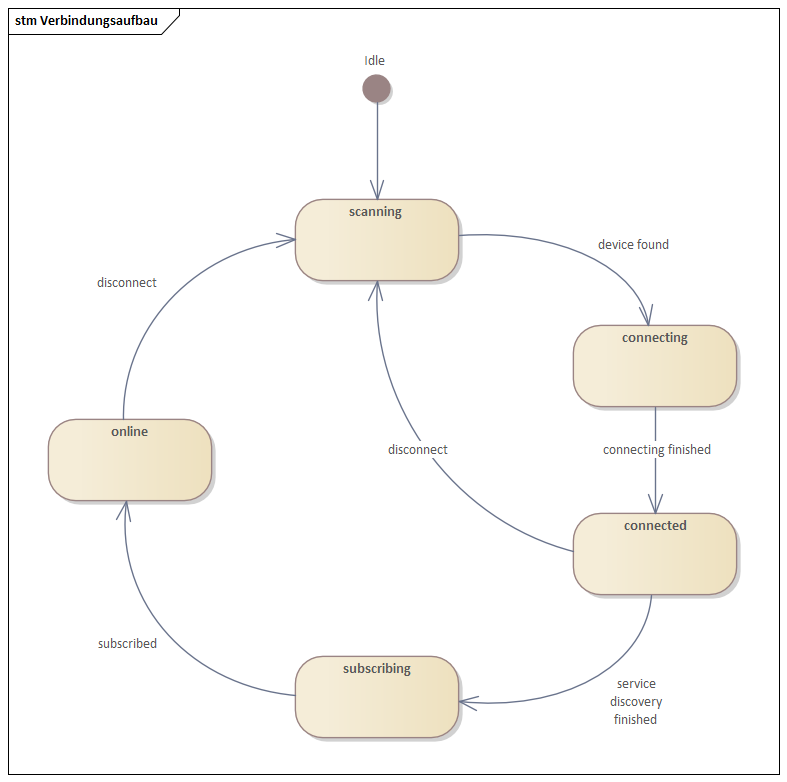
\includegraphics[width=\textwidth]{figures/Verbindungsaufbau.png}
	\caption{Zustandsdiagramm des Verbindungsaufbaus}
	\label{fig:ZustandsdiagrammVerbindungsaufbaus}
\end{figure}



\subsubsection{Optimierung Abfrage Messeinheit}
\label{OptimierungAbfrage}
Im Ausgangszustand der \ac{USB}-Dongle App muss die Anwendung bei Werkzeugen der Marke Holex jedes Mal, wenn sie ein Messergebnis erhält, die Einheit der Messung abfragen. Bei Drehmomentschlüsseln der Marke Garant wird ein Datenblock mit der Messeinheit kurz nach Erhalten des Messergebnisses empfangen. Diese Nachricht bezieht sich jedoch auf die derzeitig eingestellte Messeinheit, welche im Fall eines Arbeitsablaufs mit sich ändernden Einheiten, die Einheit für die nächste Messung ist. In diesem Fall gibt die \ac{USB}-Dongle App die falsche Einheit aus. Bei Geräten der Marke Holex wird nur bei einer Änderung der Messkonfiguration, diese übermittelt.\\
In beiden Fällen sendet das Werkzeug automatisch bei einer Änderung der Messkonfiguration einen Datenblock mit der Messeinheit an die Subscriber der \ac{HCT}-Charakteristik. Die Kontrolle der Messeinheit kann daher verbessert werden, indem die derzeitig eingestellte Messeinheit nach dem Verbindungsaufbau einmal abgefragt wird und für jedes verbundene Gerät gespeichert wird. Bei einer Änderung der Messeinheit erhält die Dongle-App die neue Messkonfiguration und aktualisiert die gespeicherte Einheit. Der Messablauf ist schematisch in Abbildung \ref{fig:Messablauf} zu sehen. Dadurch wird eine fehlerhafte Einheit in der Ausgabe vermieden. Zusätzlich dazu wird damit die Anzahl an Nachrichten der Dongle-App an das Messgerät verringert und die kritischen Ressourcen Rechenleistung und Energie geschont.

\begin{figure}[H] 
	\centering
	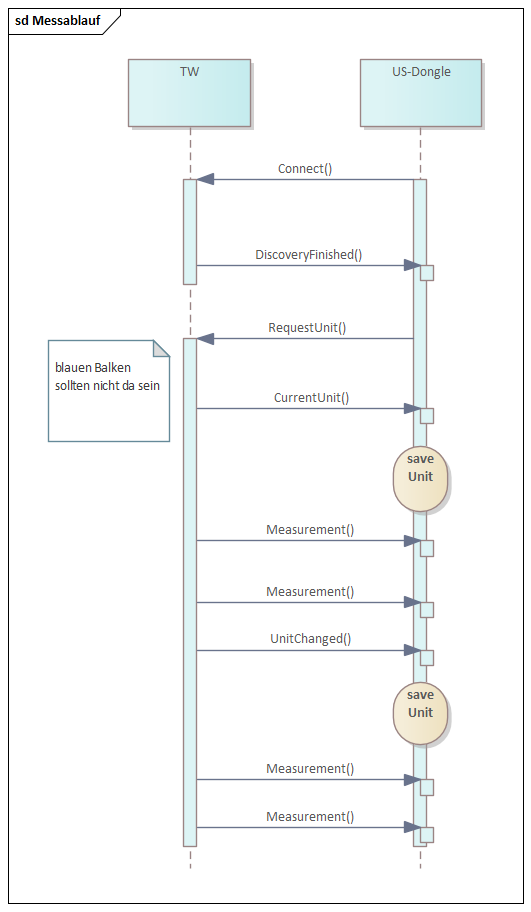
\includegraphics[width=0.65\textwidth]{figures/Messablauf.png}
	\caption{Messablauf}
	\label{fig:Messablauf}
\end{figure}

\subsection{Messmodi}
\label{Messmodi}
In diesem Kapitel werden die implementierten Messmodi vorgestellt und die Herausforderungen der Umsetzung beschrieben. Zum Ende dieser Arbeit sind folgende Modi konfigurierbar:
\begin{itemize}
	\item 0: \ac{USB}-\ac{HID}-singleKey
	\item 1: \ac{USB}-\ac{HID}
	\item 2: \ac{CDC} (COM-Port)
	\item 3: \ac{BLE}-\ac{HID}
	\item 4: \ac{BLE}-\ac{HID}-singleKey
\end{itemize}
Die Messmodi werden in die Kapitel \ac{USB}-\ac{HID} und \ac{BLE}-\ac{HID} zusammengefasst und es wird auf den Modus \ac{BLE}-Windows-App eingegangen, der vorerst nicht umgesetzt wird, jedoch für eine spätere Version geplant ist. Der Modus \ac{CDC} war zu Beginn dieser Arbeit bereits implementiert. \\
Zum Zeitpunkt der Implementierung der Dongle-App, war diese die oberste Abstraktionsschicht aller USB-Funktionalitäten. Mit Einführung der Messmodi, werden diese der Dongle-App übergeordnet. Daher muss eine neuen Abstraktionsschicht geschaffen werden, die über der Dongle- und Fußschalterapp steht und deren verschiedenen Funktionalitäten dirigiert. Dadurch können die Operationsmodi programmatisch getrennt werden, sodass bestimmte Schritte der Initialisierung nur in den bestimmten Messmodi durchgeführt werden müssen. So kann das Einlesen der Konfigurationsdatei der zu verbindenden Geräte, in einem Modus, wie \ac{HID} einzelnes Zeichen, ausgelassen werden. Außerdem lässt sich die Anwendung durch die neue Abstraktionsschicht leicht um neue Messmodi erweiterbar. Wie sich diese neue Abstraktionsschicht in das Gesamtprojekt einfügt ist in Abbildung \ref{fig:NeueAbstraktionsschicht} zu sehen.

\begin{figure}[H] 
	\centering
	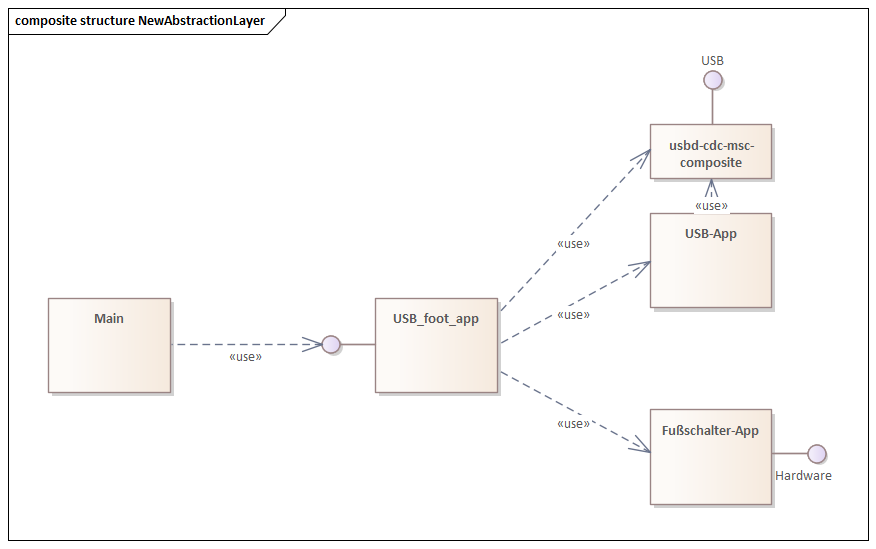
\includegraphics[width=\textwidth]{figures/NewAbstractionLayer.png}
	\caption{Neue Abstraktionsschicht}
	\label{fig:NeueAbstraktionsschicht}
\end{figure}

\subsubsection{USB-HID}
Ein Feature, das sowohl für den Dongle als auch für den Fußschalter implementiert wird, ist das Human Interface Device (HID) über USB. In diesem Modus gibt die Anwendung die Messergebnisse nicht mehr über den virtuellen COM-Port aus, sondern ist über einen \ac{USB}-Port als Tastatur mit dem Computer verbunden. Über die Tastatur werden die Zeichen der Messung als Tastendrücke, gefolgt von einem konfigurierbaren Terminierungszeichen, ausgegeben. Dadurch können Messungen in einem Tabellen Programm oder einem Texteditor aufgefangen werden.\\
Für die Implementierung werden die Funktionen des NRF-Library Files app\_usb\_hid\_kbd.h verwendet, welches die Low-Level \ac{USB}-Aufrufe abstrahiert und Funktionen zur Verfügung stellt, die bei Aufruf eine Taste drücken oder loslassen (\cite{NRF_USB_HID_keyboard}). Dabei fehlt jedoch eine Funktion die den ganzen String eines Messergebnis serialisiert, weshalb diese implementiert werden muss. Die Scancodes, die Nummern der Tasturtasten sowie der Modifier, eine Taste die Tastendrücke modifiziert, wie die Shift-Taste, werden dabei von einer Funktion erhalten, die im nrf\_Base Projekt enthalten ist. Diese Funktion ist für die \ac{HID} Implementierung über \ac{BLE} geschrieben und gibt den Scancode und zugehörigen Modifier für einen \ac{ASCII} Character zurück.\\
Zwischen den Tastendrücken muss eine gewisse Zeit gewartet werden, da der Computer Tastendrücke, zwischen denen zu wenig Zeit verstreicht, nicht registriert. Dieser Delay wird auf eine Millisekunde festgelegt, was der maximalen Übertragungsrate über \ac{USB} entspricht (\cite[17]{HID_USB_Specification}). Zudem nahm bei einem längeren Delay die Anzahl an fehlerhaften Tastendrücken zu. Diese statische Art auf eine Registrierung der Tastendrücke durch den Computer zu warten, stellt sich als sehr fehleranfällig heraus. Nicht nur wurden doppelte Zeichen nicht korrekt erkannt, sondern nach zehn Ausgaben schien der \ac{USB}-Bus überlastet zu sein und die Ausgabe der Messergebnisse bricht ab. Daher muss die Implementierung geändert werden. Statt die Tastendrücke ohne Rücksicht auf die zugehörigen Events dem \ac{USB} zu übergeben, muss nach jedem Zeichen auf ein Event der \ac{USB}-\ac{HID} Library gewartet werden, das die erfolgreiche Übertragung signalisiert. Dazu muss der zu serialisierende String in einem Buffer hinterlegt und bei Empfangen des Events das nächste Zeichen übertragen werden.\\
Eine Abwandlung dieses Modus ist der Modus \ac{USB}-\ac{HID}-singleKey. In diesem Modus gibt der Fußschalter bei Betätigung des Tasters nur ein einzelnes konfigurierbares Zeichen aus, beziehungsweise bei einem Doppelklick ein Zweites, wie in Abschnitt \ref{FußtasterFunktionalität} beschrieben ist.

\subsubsection{BLE-HID}
Ein weiterer Modus, in dem der Fußschalter arbeiten soll, ist \ac{HID} über \ac{BLE}. Dabei simuliert der Fußschalter oder Dongle eine über \ac{BLE} verbindbare Tastatur und serialisiert nach dem Verbinden wie bei \ac{HID} über \ac{USB} die Messergebnisse als Tastendrücken. Der Fußschalter muss daher nun zusätzlich zur Central Rolle in der Peripheral Rolle agieren. Dazu muss einerseits das Advertising korrekt konfiguriert werden und in den bestehenden Code des peripheren Verbindungsaufbaus, die Fußschalter Applikation, eingebunden werden. Für das Schreiben des Messergebnisses über \ac{BLE}, steht bereits eine Funktionen des nrf\_Base Projekts zur Verfügung, die einen String vollständig serialisiert und diese muss in der Fußschalter Applikation aufgerufen werden.\\
\ac{HID} über \ac{BLE} muss dabei verschlüsselt sein, mindestens mit LE-Legacy also der Option ``Just Works''. Dazu müssen die Geräte gebondet werden, damit weiteren Verbindungaufnahmen der Schlüsselaustausch nicht mehr mitgehört werden kann. Diese Bonding-Informationen werden auf dem Computer und dem \ac{BLE}-Modul gespeichert (\cite[78]{HID_BLE_Specification}). Dadurch entsteht die Anforderung, dass die Bonding Informationen der Verbindung auch wieder gelöscht werden können. Werden die Bonding Informationen auf dem Computer, jedoch nicht auf dem Fußschalter, gelöscht, können sich die beiden Geräte nicht mehr miteinander verbinden. Das muss zum Beispiel geschehen, wenn der Fußschalter mit einem anderen Computer verbunden werden soll, sich der erste Computer jedoch noch in Reichweite befindet. Trotzdem sollen nicht bei jedem Reset des Fußschalters, also bei einer Änderung der Konfigurationsdatei, die Bonding Informationen gelöscht werden, da sonst bei jedem Verbinden, der Fußschalter im Computer erst entkoppelt und dann wieder neugekoppelt werden muss. Daher kann also nicht direkt gesagt werden wann die Bonding Informationen gelöscht werden sollen und wann nicht, stattdessen wäre der Idealfall, dass der User selbst die Informationen löschen kann. Das ist aufgrund der begrenzten Interaktionsmöglichkeiten des Users mit dem Fußschalter nur schwierig umsetzbar. Ein Kompromiss ist, dass die Bonding Informationen gelöscht werden, wenn der Modus \ac{BLE}-\ac{HID} verlassen wird. Der Anwender kann dann auch um die Bonding Informationen zu löschen aus dem Modus 3 herauswechseln und dann wieder hineinwechseln. Dabei ist das Problem, dass bei einem Reset nicht direkt ersichtlich ist, in welchen Modus gewechselt wird, da die Konfigurationsdatei erst beim Neutstart neu gelesen wird. Daher wird direkt vor dem Reset die Konfigurationsdatei gelesen und falls aus dem Modus 3 oder 4 in einen anderen Modus gewechselt wird, die Bonding Informationen gelöscht. Ein alternativer Lösungsansatz, der ohne das ressourcenfordernde Einlesen der Datei auskommt, ist die Bonding Informationen immer zu löschen, wenn sich der Fußschalter beim Reset in einem anderen Modus als 3 oder 4 befindet. Allerdings ist der ``Peer Manager'' dann nicht initialisiert, der zum Löschen der Bonding Informationen zwingend benötigt wird, weshalb dieser Lösungsansatz nicht umgesetzt werden kann. Der Peer Manager ist dabei eine Library von NRF, die sich um Verschlüsselung, Pairing und Bonding kümmert (\cite[]{NRF_PeerManager}).\\
Erste Tests zeigen, dass die Geschwindigkeit der Übertragung, einerseits die Dauer bis zum ersten Tastendruck und anderseits die Zeit zwischen den einzelnen Tastendrücken, zu hoch ist. Die Untersuchung wo genau zuviel Zeit verwendet wird, fand mithilfe eines Oszilloskops und dem Toggeln eines freien Pins, der zu diesen Debugzweck belegt wurde, statt. Dadurch konnte bereits ein Bug im nrf\_Base Projekt identifziert und behoben werden. Dabei wird in der Funktion, zwischen den einzelnen Zeichen eine Pause gemacht, um ähnlich im Modus USB-\ac{HID} dem Betriebssystem Zeit zu geben die Tastendrücke zu verarbeiten. Dieser Delay ist abhängig von Connection Interval, welches wenn nur die Verbindung zum Computer besteht, korrekt gesetzt ist. Dabei stellte sich heraus, dass diese globale Variable von allen Verbindungen überschrieben wird. Diese Variable ist jedoch auch unabhängig von der \ac{HID} Funktionalität nur für die peripheren Verbindungen von Bedeutung und das Überschreiben der Variable ein Fehler. Daher wurde an der Stelle, an der diese Variable durch einen ``Connection Update Request'' überschrieben wird, die Unterscheidung eingeführt, ob die Verbindung eine periphere Verbindung ist.\\
Auch von diesem Modus, steht eine die Abwandlung \ac{BLE}-\ac{HID}-singleKey zur Verfügung, die, wie im Modus USB-\ac{HID}-singleKey, ein einzelnes Zeichen bei Betätigung des Tasters ausgibt.


\subsubsection{BLE-Windows-App}
Der letzte Modus, in dem der Fußschalter agieren soll, ist als ein an die \ac{HCT}-Windows-App angebundenes Gerät. Dabei soll das Signal der Betätigung des Tasters als eine \ac{HCT}-Nachricht an die Windows-App gesendet werden, welche dann ein Messergebnis bei den mit ihr verbundenen Messgeräten triggert. Dazu muss ein \ac{HCT}-Model für den Fußschalter geschaffen werden. Das Model stellt folgende Werte bereit:
\begin{itemize}
	\item Device Class
	\item Protocol type, version 
	\item Version of Hardware, Software, \ac{BLE}
	\item Battery level, status
	\item Reset 
\end{itemize}

Werte des Config.ini Konfigurationsfiles:
\begin{itemize}
	\item Operating Mode 
	\item \ac{CDC} protocol 
	\item HID Keyboard Language ID 
	\item HID data set seperator 
	\item HID number seperator
	\item HID single key single press
	\item HID single key double press
	\item Inactivity timeout
	\item sequentiel group triggering 
\end{itemize}

Für die Übertragung des eigentlichen Signals, dass der Fußschalter betätigt wurde, wird eine \ac{HCT}-Charakteristik angelegt, auf welche die \ac{HCT}-Windows-App subscriben kann. Über diese Charakteristik wird die App dann über die Betätigung des Tasters notifiziert. Im Advertising muss sich der Fußschalter dann nicht als Tastatur, sondern als \ac{HCT}-Fußschalter erkenntlich zeigen.\\
Dieser Modus wird erst in einer späteren Version des Fußschalters implementiert, wie im Abschnitt 8.2 genauer erklärt wird.

\subsection{Überarbeitung des MSC}
\label{UberarbeitungMSC}
In diesem Kapitel wird aufgezeigt, durch welche Schritte die finale Lösung zur Detektion einer Änderung der Konfigurationsdateien enstanden ist.

\subsubsection{Evaluierung der Möglichkeiten zur Detektion}
Der erste Versuch, der unternommen wird um dem Anwendungsfall gerecht zu werden, ist über die File Information des \ac{FAT} Filesystems den Änderungszeitpunkt auslesen. Falls er sich im Vergleich zum Zeitpunkt, der beim erstmaligen Einlesen festgestellt wurde, geändert hat, wird ein Systemneustart durchgeführen. Dabei ist hervorgekommen, dass eine Änderung an der Datei keine Veränderung am Änderungszeitpunkt hervorruft. Erst nach einem manuellen Reset ist das korrekte Änderungsdatum in der File Information abzulesen. \\
Ein weiterer Versuch besteht darin, direkt zu überprüfen, ob neue Daten über das Blockdevice geschrieben wurden. Das Blockdevice ist dabei eine Zwischenschicht zwischen Filesystem und dem physischen Speicher(\cite{NRF_Block_device}). Das führt jedoch dazu, dass der Systemneustart durchgeführt wird, bevor alle Daten vollständig geschrieben sind. Zudem hat diese Implementierung weitere Nachteile, wie zum Beispiel, dass ein Formatieren des Datenträgers, wie er bei der ersten Inbetriebnahme durchgeführt werden muss, nicht mehr möglich ist. \\
Ein periodisches Neueinlesen der Daten war hingegen nicht möglich, weil beim Lesen der Daten die Anwendung in einer Warteschleife festhängt. Das liegt daran, dass sowohl \ac{MSC} als auch das \ac{FAT} Filesystem auf die gleiche Instanz des Blockdevice versuchen zuzugreifen, was grundsätzlich nicht möglich ist. Ein Anlegen einer weiteren Instanz des Blockdevice für das Filesystem behob dieses Problem. Der schematische Aufbau der Komponenten die für das Massenspeichermedium benötigt werden, ist in Abbildung \ref{fig:KomponentenMasspeichermedium} zu sehen.\\
In einer zwischenzeitlichen Lösung des Problems werden die Konfigurationsfiles periodisch neugelesen und über die Daten ein Hashwert gebildet. Anhand dieses Wertes wird dann eine Änderung festgestellt. Ist das globale Konfigurationsfile geändert worden, wird ein Systemreset durchgeführt, während bei einer Änderung des Files der zu verbindenden Geräte, die Verbindung zu allen Geräten getrennt wird und das File anschließend neueingelesen wird. Darauf folgt ein Neustart des Verbindungsaufbauprozess. Jedoch wurde bei dieser Implementierung Änderungen, die am Ende der Datei stattgefunden haben, nicht detektiert werden. Durch eine genaue Analyse des Prozesses kann festgestellt werden, dass die Länge der Datei nicht erneut eingelesen wird, wenn die Datei aus dem Massenspeichermedium und nicht aus dem Filesystem auf dem Chip heraus geändert wurde. Daher können Änderungen an den Dateien, die ausschließlich hinten an dem bestehenden Text angefügt werden, nicht detektiert werden, da die Datei mit der alten Länge eingelesen wird.

\begin{figure}[H] 
	\centering
	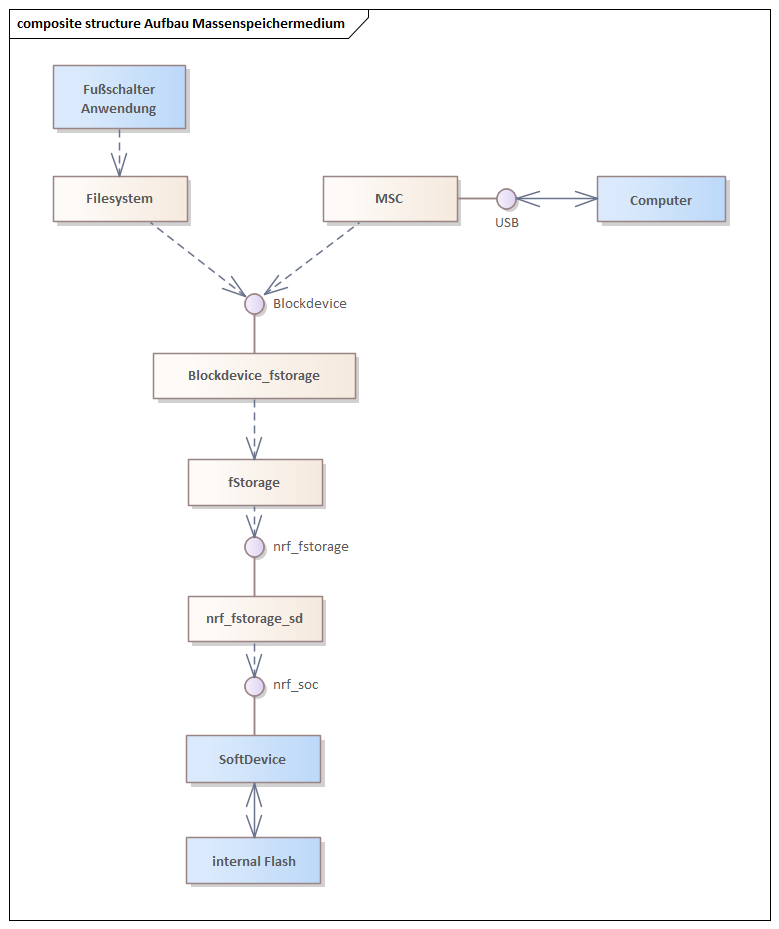
\includegraphics[width=0.8\textwidth]{figures/Aufbau_Massenspeichermedium.png}
	\caption{Komponenten des Masspeichermedium}
	\label{fig:KomponentenMasspeichermedium}
\end{figure}

\subsubsection{Manuelles Einlesen des Änderungszeitpunkts}
Durch eine manuelle Überprüfung der Daten im Speicher kann festgestellt werden, dass die Information, wie lang die Konfigurationsdatei ist, korrekt im Speicher vorhanden ist, aber nicht ins interne Filesystem übernommen wird. Daher besteht die Möglichkeit die Informationen selbstständig einzulesen. Dazu muss als Erstes das ``Directory Entry'' gefunden werden, welches nach den \ac{FAT} steht und die Informationen zur Datei beinhaltet, wie die Länge in Bytes und das Änderungsdatum (\cite[Abschnitt 1.4]{FAT}). Daher müssen folgende Informationen aus der Boot Section ausgelesen werden und folgende Berechnung durchgeführt werden:
\begin{itemize}
    \item Sa: Startadresse Filesystem
    \item Sg: Sektorengröße
    \item nrS: Anzahl reservierter Sektoren
    \item nF: Anzahl \ac{FAT}
    \item nSF: Anzahl Sektoren pro \ac{FAT}
\end{itemize}

\[Sa + Sg \cdot nrS + Sg \cdot nF \cdot nSF = Sa + Sg\cdot(nrS + nF \cdot nSF)\]

Diese Informationen stehen immer an der gleichen Stelle im Bootsektor und werdem während des Betriebs des Fußschalters nicht verändert. \\
Im Directory Entry wird jeweils für die Informationen einer Datei 32 Bytes verwendet und innerhalb dieser 32 Bytes befinden sich die Informationen immer an der gleichen Stelle, weshalb mit festen Offsets gearbeitet wird. Der Eintrag wird aber nicht sofort gelöscht, wenn die Datei gelöscht wird, sondern die Filenamen durch Ersetzten des ersten Buchstaben durch 0x5a invalidiert (\cite[Abschnitt 1.4]{FAT}). Daher muss der valide Eintrag immer wieder neu gesucht werden. Dadurch kann das Directory Entry größer als ein Sektor werden, auch wenn es nur zwei Dateinamen beinhaltet. Daher werden nacheinander die Sektoren, die für das Directory Entry allokiert sind, eingelesen und auf die korrekten Dateinamen hin untersucht. Ist der korrekte Eintrag gefunden, wird der Änderungszeitpunkt eingelesen und nach der bereits beschriebenen Methode überprüft. Hier wird wieder der Änderungszeitpunkt zur Detektion einer Änderung verwendet, da die Länge der Datei nur dazu benutzt werden kann, die Datei ``händisch'' einzulesen, also direkt über Flash Zugriffe und nicht über die \ac{FAT} Filesystem Library. Was kurzzeitig in Angesicht der weiterhin bestehenden Probleme in Erwägung gezogen wird, aber aufgrund des hohen Entwicklungsaufwands als zu vermeiden eingeordnet wird. Dabei kann aus dem Directory Entry auch der Startsektor der Datei ausgelesen werden und ähnlich der Adresse des Directory Entry, die Adresse des Sektors berechnet werden. Auf den ersten Blick erscheint das nicht kompliziert, allerdings wird die Datei, falls sie größer als ein Sektor wird, auf nicht zwangsläufig aufeinanderfolgende Sektoren verteilt, was nur anhand der \ac{FAT} nachvollzogen werden kann. Um eine korrekte Funktionsweise des Fußschalters auch bei einer wachsenden Konfigurationsdatei zu garantieren, müsste ebenfalls das Auslesen der \ac{FAT} implementiert werden.

\subsubsection{Finale Lösung}
Das Hauptproblem des \ac{MSC} ist, dass es immer wieder dazu kommt, dass Schreibbefehle fehlschlagen und die Daten unvollständig in den Speicher übertragen werden. Dabei wurde davon ausgegangen, dass die Schreibbefehle fehlschlagen, weil der Neustart des Fußschalters zu früh erfolgt und die zu schreibenden Daten nicht vollständig in den Speicher übertragen wurden. Schließlich wurde ersichtlich das dies eine grundlegende Fehlannahme ist und stattdessen ergeben Nachforschungen, dass die Zugriffe auf den Flash vom Softdevice abgearbeitet werden müssen und dass aufgrund der mehrere aktiven Verbindungen die Wahrscheinlichkeit von Fehlerhaften Schreibzugriffen stark ansteigt (\cite[Abschnitt SoftDevice Backend]{NRF_fstorage}). Die getätigte Änderungen an den Konfigurationsfiles werden dann nicht übernommen und sind selbst nach langen Wartezeiten, nach dem Reset verloren. Deshalb werden, falls Schreibzugriffe gequeuet sind, alle Aktivitäten des Softdevice gestoppt, um die Gefahr von Fehlern beim Schreiben und die benötigte Zeit zu minimieren. Das umfasst das Trennen aller Verbindungen sowie das Stoppen von Advertising und Scanning. Da durch einen gestarteten Timer der Fußschalter ohnehin neugestartet werden soll, damit die Konfigurationsfile neueingelesen werden können, ist die Beeinträchtigung der User Experience vernachlässigbar.\\
Diese Problematik besteht auch im Modus \ac{BLE}-\ac{HID}, da die Bonding Informationen über dieselbe Library vom Softdevice in den Flash geschrieben werden (\cite{NRF_PeerManager}). Ist der Fußschalter zum Zeitpunkt des Verbindens mit dem Computer bereits mit mehreren Werkzeugen verbunden, besteht eine hohe Wahrscheinlichkeit, dass die Bonding Informationen fehlerhaft geschrieben werden. Der Fußschalter kann sich dann nicht mehr mit dem Computer verbinden, beziehungsweise kann dieser keine Zeichen über einer bestehenden Verbindung übertragen. Die Lösung dieses Problems besteht darin, das Verbinden des Werkzeugs erst zu starten, wenn die periphere Verbindung zum Computer bereits besteht. Da ohne die Verbindung zum Computer dieser Modus nicht nutzbar ist, ist die Userexperience dadurch nicht beeinträchtigt.

\subsection{Einbindung Messuhren}
\label{EinbindungMessuhren}
In der Vorbereitung auf die Implementierung der fußschalterspezifischen Features wird die Dongle-App um die Unterstützung der Messuhren bzw. Messschieber erweitert, da sich die meiste Funktionalität des Fußschalters speziell auf die Messuhren bezieht. Messuhren und Messschieber sind in diesem Kontext dabei gleichbedeutend, weil das \ac{HCT}-Interface für beide Geräte identisch ist. Nachfolgend wird sich daher stets auf Messuhren bezogen.

\subsubsection{Unterscheidung der Geräte}
Im einfachsten Anwendungsfall ist der Fußschalter mit mehreren Werkzeugen verbunden und sammelt passiv deren Messergebnisse ein. Unabhängig vom eingestellten Messmodus benötigt die Dongle-App von den Geräten einerseits das Messergebnis und andererseits die Messeinheit, um die Ergebnisse vollständig an den Computer weitergeben zu können. Diese befinden sich abhängig vom Gerät an folgenden \ac{HCT}-Protokoll-Adressen:

\begin{table}[H]
	\centering
	\begin{tabular}[H]{l|l|l}
		 & Datenblock & Adresse \\
		\hline
		Garant Drehmomentschlüssel & & \\
		Messergebnis & Measurement data block & 0x00000B04 \\
		Messeinheit & Setpoint data block & 0x00000C1F \\
		\hline
		Holex Drehmomentschlüssel & & \\
		Messergebnis & Device measurement result & 0x0000240C \\
		Messeinheit & Device measurement case config & 0x0000221B \\
		\hline
		Messuhren/Messschieber & & \\
		Messergebnis & Device measurement result & 0x00002408 \\
		Messeinheit & Device measurement case config & 0x0000220F \\
	\end{tabular}
	\caption{Adressen Messergebnis und Messeinheit}
\end{table}

In Tabelle 1 wird deutlich, dass die Adressen von Messergebnis und Messeinheit für diese drei Geräte jeweils unterschiedlich sind, auch wenn sie im Fall der Messuhren und Holex Drehmomentschlüssel im gleichen Datenblock liegen. Wird dieser als Binärdaten erhalten kann die Adresse des Datenblocks gelesen werden, die Information von welchem Gerät die Daten stammen und damit an welcher Stelle genau die Daten jeweils zu finden sind, kann jedoch nicht festgestellt werden. Diese Problem kann vermieden werden indem ein Library der Hoffmann Group eingesetzt wird, die ``BLE Proxy Library''. Diese stellt Funktionen zur Verfügung, welche eine Zuordnung der Daten in die dazugehörenden Strukturen übernimmt, sowie die Daten vollständig serialisieren und deserialisieren kann. Die Möglichkeit wurde jedoch ausgeschlossen, da vorrausgesetzt wird, dass ein vollständiges Schnittstellendatenmodell der verbundenen Geräte im Speicher vorgehalten wird, während der Fußschalter nur wenige spezifisiche Daten benötgigt. Daher bleibt keine andere Möglichkeit als die verbundenen Geräte ihrem Typ zuzuordnen und die erhaltenen Daten entsprechend zu interpretieren.\\
Diese Unterscheidung mit welcher Art von Gerät kommuniziert wird, kann auf zwei verschieden Weisen erfolgen. Einerseits kann anhand des Namens das Gerät entweder der Klasse Drehmomentschlüssel oder Messuhr zugeordnet werden. Das ist unter Umständen fehleranfällig, da das Sortiment an \ac{HCT}-Werkzeugen stetig wächst und es nicht auszuschließen ist, dass in der Zukunft Geräte auf den Markt kommen, mit deren Namen es zu falschen Zuordnung kommt. Zudem sind alte Messschieber im Umlauf, die zwar unter einem korrekten Name advertisen aber nicht das \ac{HCT}-Protokoll sprechen, wobei diese Geräte aufgrund der Inkompatibilität der Protokolle letztendlich nicht verbunden werden können.\\
Eine andere Methode ist, die ``Device Information'' abzufragen und anhand der Klassenidentifikationsnummer das Gerät einem Typ zuzuordnen. Das ist die präferierte Lösung, da neben der genaueren und sicheren Zuordnung in der Device Information andere Informationen, wie die Protokoll Version mitgeliefert werden, die bei späteren Features benötigt werden. Zudem bleibt die Datenverarbeitung leichter erweiterbar um neue Geräte. Diese Abfrage muss in den asynchronen und mehrteiligen Ablauf des Verbindungsaufbaus eingefügt werden, wodurch ein höherer Entwicklungsaufwand entsteht. Auch benutzen Drehmomentschlüssel der Marke Garant eine andere Klassifikation der Geräte als das Werkzeug der Marke Holex, welche innerhalb der Dongle-App vereinheitlicht werden muss.\\
Da die Erweiterbarkeit und die Flexibilität dem höheren Entwicklungsaufwands überwiegen, fällt die Entscheidung auf diese Lösung. Dabei wird nach dem Verbindungszustand-Callback, der vom Central Device nach einer erfolgreichen Subscription der Anwendung auf die \ac{BLE}-Charakteristik des Werkzeugs aufgerufen wird, eine Nachricht zur Abfrage der Device Information gesendet. Die erhaltenen Daten werden dann in der zum Gerät gehörenden Struktur gespeichert und anschließend erfolgt die Abfrage der Messeinheit. 

\subsubsection{Anpassung der Messdatenverarbeitung}
Auch die Datenverarbeitung, also die Interpretation der erhalten Daten über \ac{BLE} muss angepasst werden, da das Messergebnis, wie bereits in Tabelle 1 gezeigt, zwar innerhalb des gleichen Datenblocks wie bei dem Holex Drehmomentschlüssel liegt, jedoch innerhalb des Datenblocks an einer anderen Stelle zu finden ist. Diese Offsets sind als Konstanten im Headerfile der Dongle-App definiert und müssen um die entsprechenden Einträge für die Messuhren erweitert werden. Werden die Daten erhalten, wird als Erstes die Adresse ausgelesen und dann je nach Typ des zugehörigen Geräts die Interpretierung der Daten durchgeführt. Beim Einbinden weiterer Geräte, können zusätzliche Sonderbehandlungen der Daten anhand des Typs hinzugefügt werden. Zudem ist das Messergebnis, das von Interesse ist, beim Drehmomentschlüssel der ``Peak Torque'', der als Gleitkommazahl codiert ist, während bei der Messuhr das Ergebnis die ``Measurement Distance'' als Ganzzahl codiert ist. Dieses ist abhängig von der Messeinheit in Mikrometer oder Mikroinch gespeichert. Das Messergebnis muss auf Millimeter beziehungsweise Inch umgerechnet werden, da die Ausgabe über \ac{CDC} oder \ac{HID} der Anzeige auf dem Gerätedisplay gleichen soll. Das binäre Messergebnis wird daher zunächst mit einem Umrechnungsfaktor von 1000 in Millimeter beziehungsweise Milliinch als Gleitkommazahl umgerechnet. Anschließend muss überprüft werden, ob die derzeitige eingestellte Einheit des Geräts Inch ist, da dann der Wert erneut durch 1000 dividiert werden muss, um von Milliinch auf die gewünschte Einheit Inch zu gelangen. Daher wird letztendlich eine Gleitkommazahl erhalten, wodurch die Zahl ohne Anpassungen in der Nachrichten Struktur der Dongle-App gespeichert wird.\\
Die Einheitenkodierung der Messuhr ist komplementär zur Kodierung der Drehmomentschlüssel. Daher kann die if-Cascade, welche die Zuordnung vornimmt, um die Einheiten der Messuhr erweitert werden. Die Information welche Einheit verwendet wird, befindet sich allerdings wie das Messergebnis, ebenfalls an einer anderen Stelle innerhalb des Datenblocks und muss entsprechend angepasst werden.

\subsubsection{Gruppenfunktion}
\label{Gruppenfunktion}
Durch das Betätigen des Fußtasters am Fußschalter wird bei allen verbundenen Messuhren das derzeitige Messergebnis abgefragt. Während im Modus 2 (\ac{CDC}) ein Messergebniss, anhand der Kanalnummer einem Werkzeug zugeordnet werden kann ist dies in den \ac{HID}-Modi nicht der Fall. Daher muss die korrekte Reihenfolge der Ausgabe der Messergebnisse sichergestellt werden. Somit wird festgelegt, das devices.csv Konfigurationsfile um eine Spalte mit einer Gruppennummer zu erweitern, da somit der Anwender sowohl die Reihenfolge, als auch welche Messuhren in der Gruppe sind, konfigurieren kann. Da durch das Abschicken der Nachrichten zur Abfrage der Messungen in der korrekten Reihenfolge, das tatsächliche Erhalten in der gleichen Reihenfolge nicht sichergestellt ist, wird davon ausgegangen, dass die Nachrichten in einer zufälligen Reihenfolge erhalten werden. Daher werden bei der Ausgabe die Nachrichten umsortiert. Dazu wird ein Zähler eingesetzt, der durch Betätigung des Fußschalters von 0 auf 1 gesetzt wird. Dadurch ist der Start der Gruppenfunktion später beim Erhalten der Messergebnisse erkennbar. Bei der Abarbeitung der erhaltenen Nachrichten wird dann, über die Zuordnung zum Device, die Nachricht ausgewählt und weitergegeben, die zum Counter korrespondiert. Die Gruppenids, die keinem der konfigurierten Geräte zugeordnet werden können, sowie die Gruppenids die zu unverbundenen Geräten gehören, werden dabei übersprungen. Zusätzlich wird ein Feature der Messeruhren genutzt, um die Gruppennummer auch auf der Messuhr anzuzeigen. Dazu werden den Messuhren ihre Gruppennummern, nach dem Verbindungsaufbau via dem \ac{HCT}-Protokoll, übermittelt.\\
Durch spätere Anregungen von Messtechnikern, die für den Vertrieb von Messwerkzeugen zuständig sind, wurde erarbeitet, dass wenn ein Gerät der Gruppe zwar konfiguriert, jedoch nicht verbunden ist, die präferierte Lösung ist die gesamte Gruppe nicht zu triggern. Diese Problematik entsteht dadurch, dass die Messuhren aufgrund ihrer relativ kleinen Batterien bei Inaktivität schnell ausgeschalten werden und somit die Verbindung zu ihrem Central trennen. Andererseits soll jede durchgeführte Messung korrekt sein, da sie durch die \ac{CAQ}-Software verarbeitet und gespeichert wird. Das Ziel der Sicherstellung einer korrekten Messung überwiegt hier also dem Gedanken der Benutzerfreundlichkeit, dass eine Messung auch dann gemacht werden kann, wenn einer der Geräte unverbunden ist. Der Fußschalter blinkt zur Fehlersignalisierung zwei Mal kurz rot auf.\\
Des Weiteren besteht die Möglichkeit, dass eine Messung zwar angefragt, aber nicht erhalten wird. Die Anwendung blockiert dann, da auf die Nachricht gewartet wird. Daraufhin muss ein Neustart erfolgen, weswegen die Entscheidung getroffen wurde, einen Timer zu starten, falls eine Nachricht nicht erhalten wird und beim Ablaufen der eingestellten Zeit, statt dem Messergebnis eine Fehlermeldung auszugeben. Die restlichen Messergebnisse werden dann korrekt ausgegeben werden.\\
Ebenfalls aus dem Feedback der Messtechniker heraus, wird ein sequentielles Triggern der Gruppefunktion implementiert. Dazu muss der entsprechende Eintrag in der Konfigurationsdatei mit einer 1 auf aktiv gesetzt werden. Bei den Geräten der Gruppe wird nacheinander, jeweils bei Betätigen des Fußtaster, die Abfrage eines Messergebnisses ausgelöst.

\subsection{Einbindung Hardware}
\label{EinbindungHardware}
Die Prototypen des Fußschalters der Firma Brecht sind bereits vor Beginn dieser Arbeit erhalten worden und somit konnte direkt mit der Inbetriebnahme der neuen Hardware begonnen werden. Der Chipsatz des Fußschalters ist ebenfalls der PCA10056 von Nordic semiconductor, somit muss an der Software des \ac{USB}-Dongles keine Änderung vorgenommen werden. In diesem Kapitel werden die hardwarebezogenen Funktionalitäten des Energiemanagements, des Fußtaster und der \ac{LED} vorgestellt. Im Anhang finden sich die ursprünglichen Hardwarezeichnungen der Platine.

\subsubsection{Energie Management}
\label{EnergieManagement}
Um den Fußschalter herunterzufahren und den Stromverbrauch zu senken, sah eine erste Idee vor das im nrf\_Base Projekt vorhandene Energiemanagement zu benutzen. Dieses fährt aus dem Main-Loop heraus getriggert den Chip bei Inaktivität des Softdevice weitestgehend herunter, wodurch der Stromverbrauch stark sinkt. Ist der \ac{USB}-Port also nicht verbunden und es wird keine Aktivität in der Fußschalter Anwendung registriert, wird ein Timer gestartet. Läuft der Timer ab, werden alle \ac{BLE}-Verbindungen getrennt und falls notwendig das Scanning und Advertising gestoppt. Bei Registrierung einer Aktivität, während der Timer aktiv ist, wird ein Neustart des Timers ausgelöst. Sobald der Fußschalter wieder über \ac{USB} verbunden wird, stoppt der Timer. Dieser Implementierung liegt die Vermutung zugrunde, dass wenn der Chip vollständig heruntergefahren wurde, er auch nicht durch Betätigung des Fußtasters wieder neugestartet werden kann.\\
Zunächst ist aufgefallen, dass bei der Hardware des Fußschalters der Akku auf der Datenleitung des \ac{USB} liegt. Dadurch werden in der Anwendung nicht, wie bei dem EvalBoard, die Events für \ac{USB} connected und \ac{USB} disconnect erhalten. Daher muss am Fußschalter eine Hardwareänderungen durchgeführt werden. Hierfür wird die Eingangsspannung bereits vorher abgegriffen und auf den Pin des Fußtasters gelegt. Der Fußtaster erhält einen unbelegten Pin. Mit einem \ac{ADC} wird dann überprüft, ob eine Spannung auf diesem Pin anliegt.\\
Die Einbindung des Fußtasters zeigt, dass die Anwendung durch Betätigung des Fußtasters selbst aus einem Shutdown heraus wieder aufgeweckt wird. Daher wird nach Ablaufen des Inaktivitätstimers die Anwendung vollständig heruntergefahren, um einen noch höheren Energieeffizienzgrad zu erreichen.

\subsubsection{Fußtaster Funktionalität}
\label{FußtasterFunktionalität}
Nach Überarbeitung der Codebasis und Einbindung der Messuhren stehen alle Funktionalitäten bereit um den eigentlichen Fußtaster einzubinden. Während bei der initialen Einbindung des Fußtasters eine Betätigung das Abfragen der Messergebnisse bei allen verbundenen Messuhren triggert, wächst die Funktionalität stetig an.\\
Zum Ende dieser Arbeit wird durch ein kurzes Betätigen oder einem ``einfachen Klick'' die bereits beschriebene Gruppenfunktion ausgeführt. Im Modus 0 (USB-\ac{HID}-singleKey) und 4 (\ac{BLE}-\ac{HID}-singleKey) wird daraufhin ein Timer gestartet, welcher derzeit auf 500ms gesetzt ist. Wird während seiner Laufezeit eine zweite Betätigung getätigt, wird ein ``Doppelklick'' registriert und das dafür in der Konfigurationsdatei hinterlegte Zeichen ausgegeben. Dadurch kann der User in diesem Modus schnell Dialogoptionen in der \ac{HCT}-Windows-App auswählen oder in einem Textfile die Seiten wechseln. In einem anderen Modus führt das Warten auf die zweite Betätigung, jedoch zu einer Verzögerung der Ausgabe um die Dauer des Timers, weshalb dort die Doppelklick Funktionalität zugunsten des Ansprechverhalten des Tasters entfällt.\\
Wird der Taster hingegen für drei Sekunden durchgängig gehalten, wird das Gerät heruntergefahren. Diese Funktionalität dient vorrangig dem Zweck der Kundenvorführung des Fußschalters im Rahmen einer Messe, da zum diesem Zeitpunkt der automatische Reset des Geräts bei Änderung der Konfigurationsfiles noch nicht implementiert war. Das einfache Herunterfahren des Fußschalters ist aufgrund des positiven Feedbacks beibehalten.

\subsubsection{Inbetriebnahme LED}
Auf dem Board des Fußschalters befindet sich eine \ac{LED}, die durch einen Lichtkanal nach außen hin durch das Gehäuse sichtbar gemacht wird und die dazu benutzt wird den internen Zustand des Geräts darzustellen. Folgende Zustände, aufgeführt in der Tabelle, sollen abgebildet werden.

\begin{table}[H]
	\centering
	\begin{tabular}[H]{l|l}
		Zustand & \ac{LED}-Farbe \\
		\hline
		Gerät im Sleep Modus & Aus \\
		\hline
		Alle zu verbindenden Geräte verbunden & Blau \\
		\hline
		Min. ein Gerät verbunden, es wird nach den fehlenden Geräten gescannt & Blau blinkend \\
		\hline
		Kein Gerät verbunden, Scanning inaktiv & Grün \\
		\hline
		Kein Gerät verbunden, Scanning aktiv & Grün blinkend \\
		\hline
		\ac{MSC}-Schreibvorgang detektiert & Gelb \\
		\hline
		Min. ein Konfigurationsfile nicht gefunden & Rot \\
		\hline
		Fehler in den Konfigurationsfiles & Rot blinkend \\
	\end{tabular}
	\caption{LED-Zustände}
\end{table}

Zudem blinkt der Fußschalter, wie in Kapitel \ref{Gruppenfunktion} beschrieben, zwei Mal kurz rot auf, wenn bei Betätigung des Fußtasters nicht alle zu der Gruppe gehörenden Geräte verbunden sind. Außerdem blinkt die Drei-Farben-\ac{LED} des Fußschalters vor einem Neustart oder dem Ausschalten des Geräts zweimal kurz grün.
